\mainmatter%
\setcounter{page}{1}

\lectureseries[\course]{\course}

\auth[\lecAuth]{Lecturer: \lecAuth\\ Scribe: \scribe}
\date{January 14, 2010}

\setaddress%

% the following hack starts the lecture numbering at 1
\setcounter{lecture}{3}
\setcounter{chapter}{3}

\lecture{Fundamental Properties of Nonlinear Systems I}

\section{Recap}
This corresponds to Chapter 3 of Khalil and is concerned with the \textit{existence} and \textit{uniqueness} of solutions to nonlinear systems of the form
$$\dot{x} = f(t,x)$$

\begin{example}
Consider
$$\dot{x} = -x + x^3$$
Then we have that $|x(t)|\to\infty$ as $t\to\tfrac{1}{2}\text{ln}\frac{x_0^2}{x_0^2-1}$ if $|x_0|>1$ as seen in Figure~\ref{fig:04nonexist}.
Recall from \S\ref{sec:01fet} that growth greater than linear can cause the non-existence of solutions.
$\lozenge$
\end{example}

\begin{figure}[ht!]
\centering
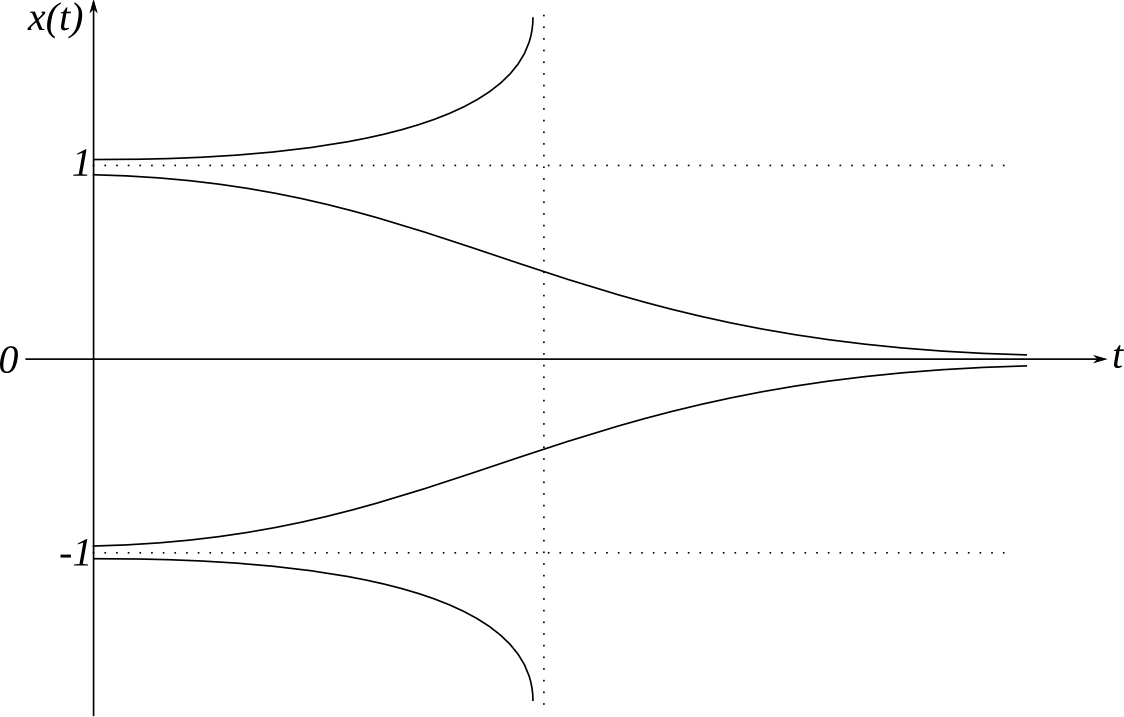
\includegraphics[width=.5\textwidth]{images/04nonexist}
\caption{System with non-existence of solution.}
\label{fig:04nonexist}
\end{figure}

\section{Uniqueness}
Uniqueness occurs when, from an initial condition, there is only a single trajectory.

\begin{example}
To see a system that has a non-unique solution consider
$$\dot{x} = \sqrt[3]{x}$$
This leads to
$$\frac{dx}{\sqrt[3]{x}} = dt \Rightarrow \tfrac{3}{2}\left(x{(t)}^{2/3}-x_0^{2/3}\right) = t$$
If $x_0\neq0$ then
$$x(t) = \text{sgn}(x_0)\left(x_0^{2/3}+\tfrac{2}{3}t\right)^{3/2}$$% chktex 3
This grows to the power of $\frac{3}{2}$ which is not quite quadratic.
If $x_0=0$ then we get multiple valid solutions including
\begin{align*}
x(t) &= 0 \\
x(t) &= \pm{(\tfrac{2}{3}t)}^{3/2}
\end{align*}
There are even more valid solutions.
For these cases we have
$$x(t) = \begin{cases} 0, & t\in[0,T]~\forall T\in[0,\infty] \\ \pm{(\tfrac{2}{3}(t-T))}^{3/2}, & t\geq T \end{cases}$$
The resulting trajectories can be seen in Figure~\ref{fig:04multsols}.
The slope is infinite at the origin so $\sqrt[3]{x}$ is not differentiable at the origin as seen in Figure~\ref{fig:04infslope}.
This leads to non-uniqueness of the solution.
$\lozenge$
\end{example}

\begin{figure}[ht!]
\centering
\includegraphics[width=.5\textwidth]{images/04multsols}
\caption{System with non-uniqueness of solution.}
\label{fig:04multsols}
\end{figure}

\begin{figure}[ht!]
\centering
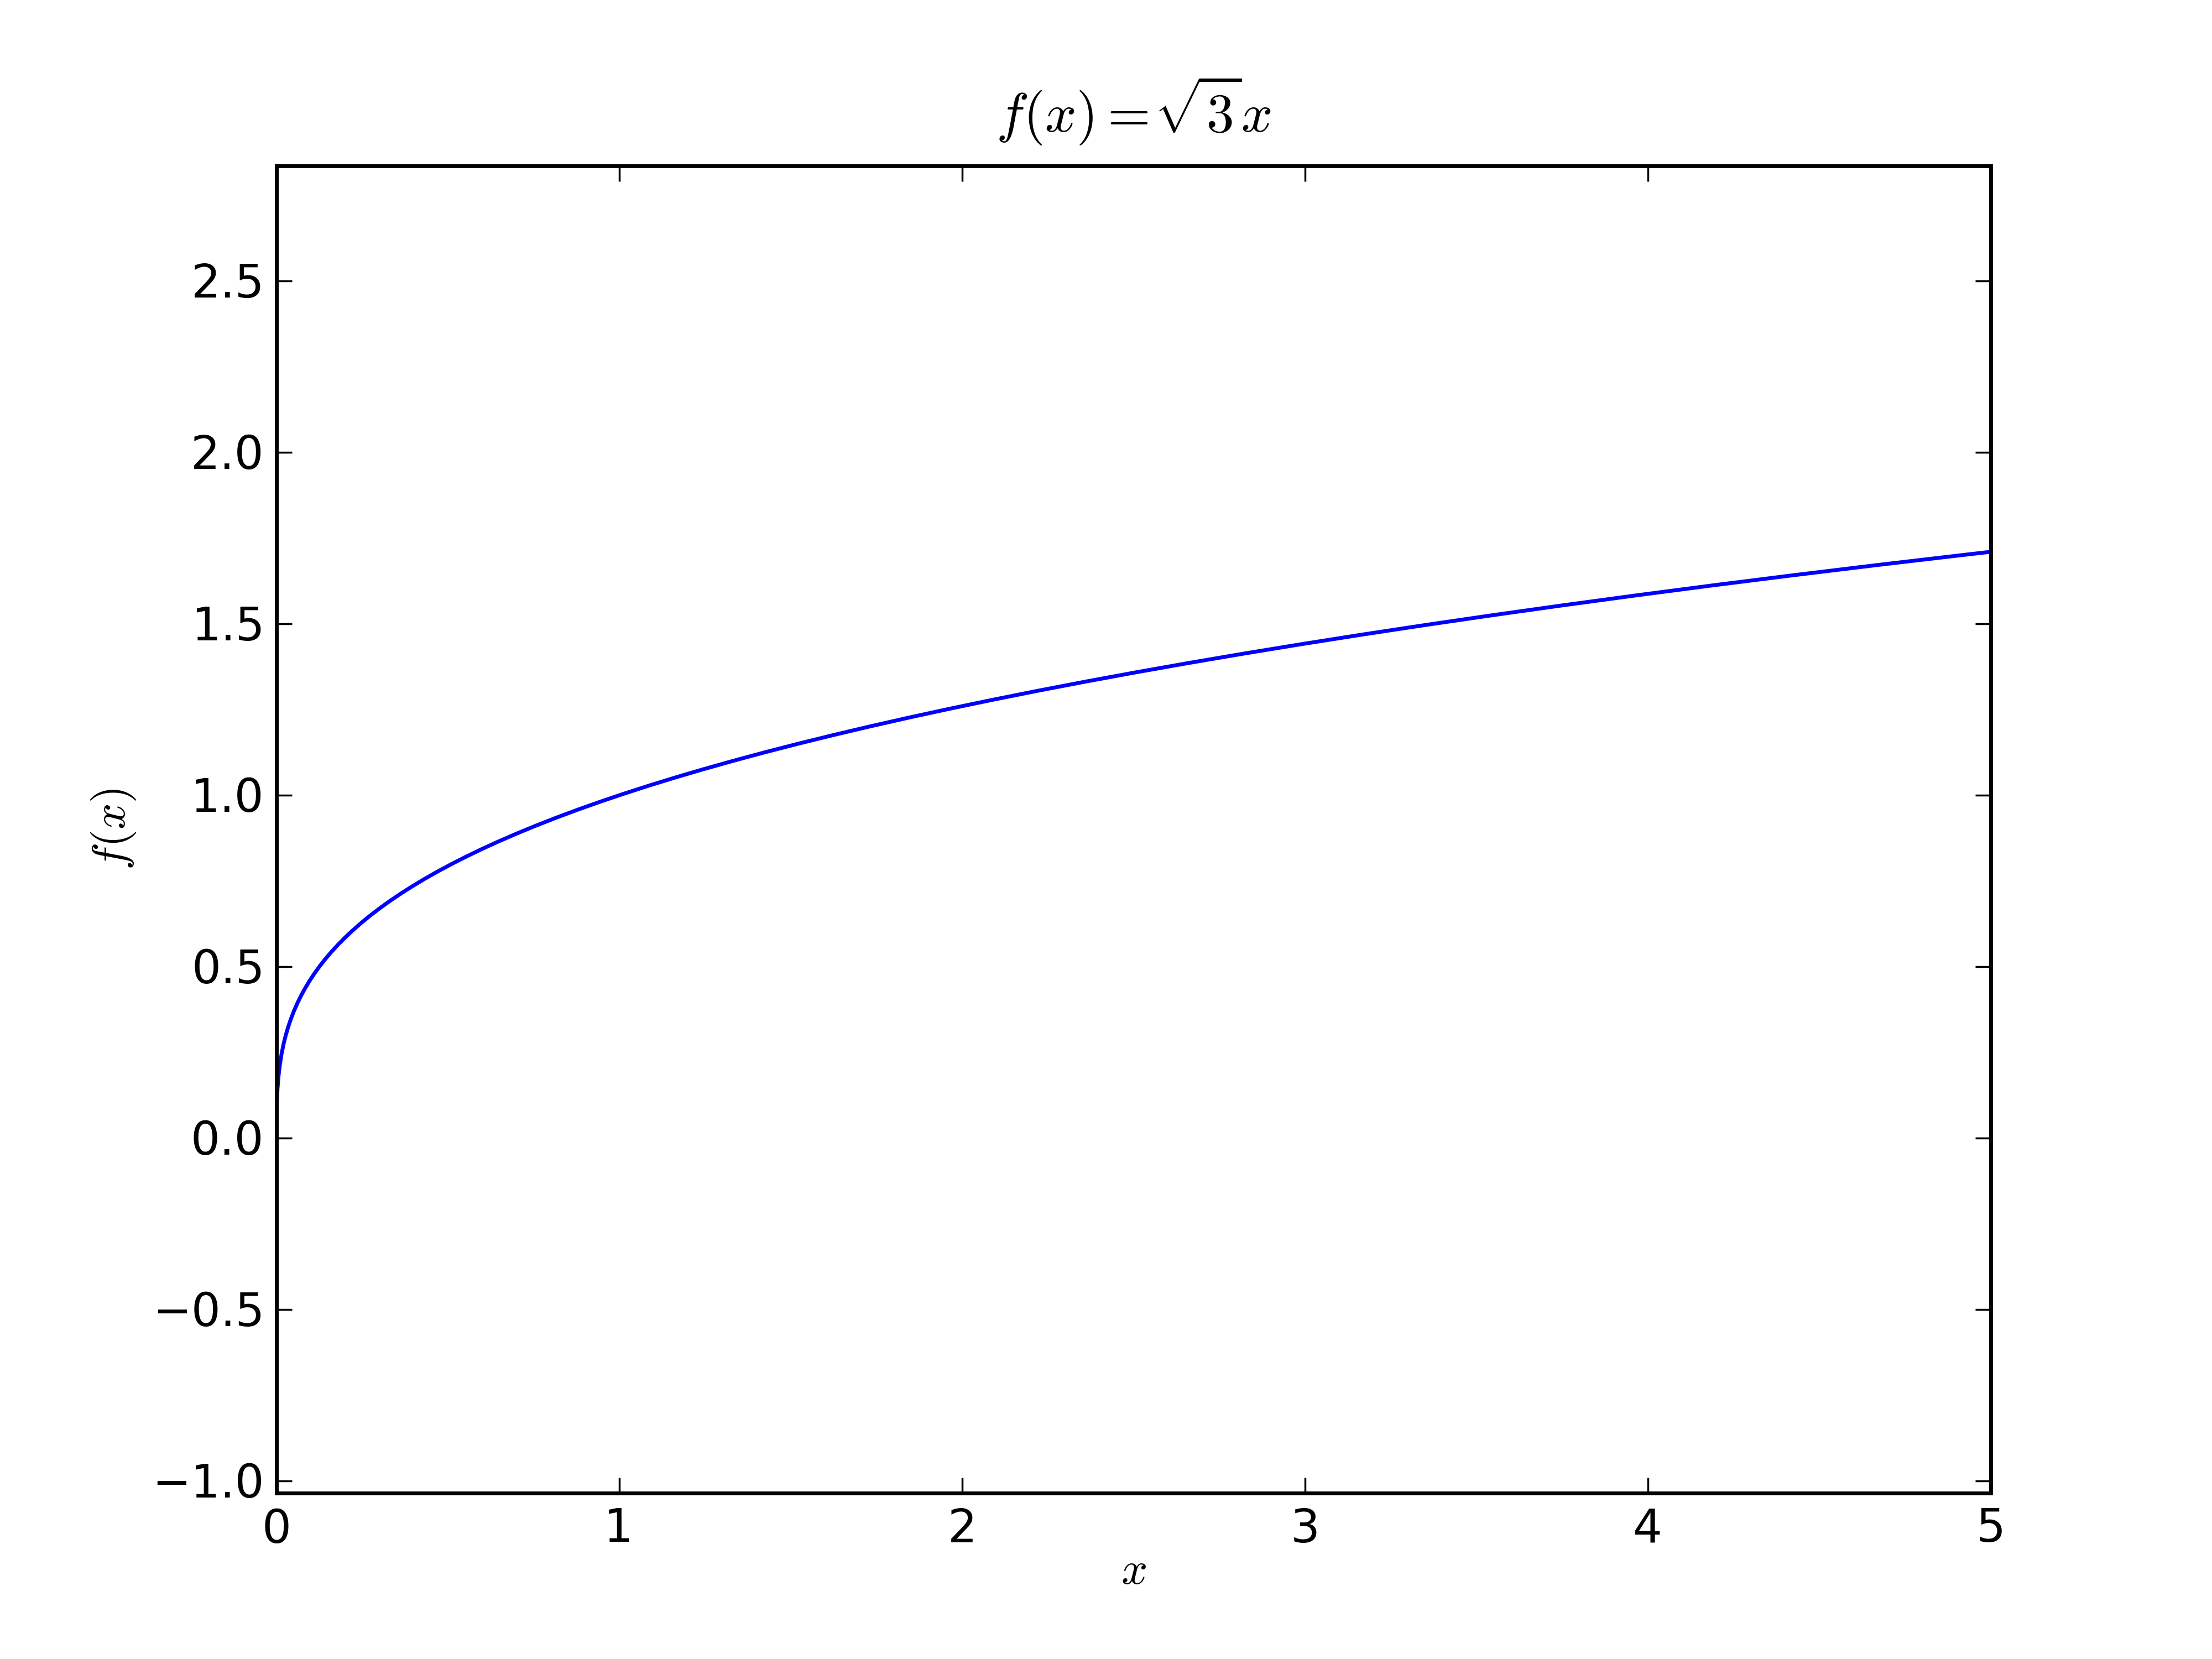
\includegraphics[width=.5\textwidth]{images/plotCubeRootX}
\caption{Plot of $f(x) = \sqrt[3]{x}$.}
\label{fig:04infslope}
\end{figure}

\section{Continuity}
Continuity deals with the $\mathcal{C}^0$ space.

\begin{definition}
A function $f(x)$ is \textit{continuous} at a point $x$ if $\forall \epsilon \exists \delta$ s.t.
$$|x-y|<\delta \Rightarrow |f(x)-f(y)|<\epsilon$$
\end{definition}
Note that Khalil uses the notation $||\cdot||$ while this course uses $|\cdot|$ to denote a Euclidean norm.
Many mathematicians save the notation $||\cdot||$ for non-Euclidean spaces such as Banach, $L_2$, $L_\infty$, etc.

\begin{definition}
A function $f$ is \textit{uniformly continuous} if $\delta$ only depends on $\epsilon$, not on $x$.
\end{definition}
Uniformly continuous refers to a global property of a function and is a stronger statement than continuous at a point.

\begin{definition}
A function $f:\mathbb{R}^n\to\mathbb{R}^n$ is \textit{continuously differentiable} $(\mathcal{C}^1)$ if $\frac{\partial f_i}{\partial x_j}$ exist and are continuous.
\end{definition}

\begin{definition}
If $f:\mathbb{R}^n\to\mathbb{R}$ then the \textit{derivative} of $f$ is
$$\frac{\partial f}{\partial x} = \left[\begin{array}{c c c} \frac{\partial f}{\partial x_1} & \cdots & \frac{\partial f}{\partial x_n} \end{array}\right]$$
\end{definition}

\begin{definition}
The \textit{gradient} of a function $f$ is
$$\nabla{} f (x) = \left(\frac{\partial{} f}{\partial{} x}\right)^T$$
\end{definition}

\begin{theorem}
The Mean Value Theorem is for a function $f:\mathbb{R}^n\to\mathbb{R}$ with a line segment given by
$$L (x,y) = \{\mathcal{Z}~|~\mathcal{Z} = \theta{} x + (1-\theta) y, 0<\theta<1\}$$
Then there exists $z\in{} L (x,y)$ such that
$$f (y)-f (x) = \left.\frac{\partial{} f}{\partial{} x}\right|_{x=z} (y-x)$$
\end{theorem}
This is similar to a Taylor series expansion.
However, it is an exact form but the derivative is evaluated not at $x=x$ but at $x=z$.
The theorem does not say what $z$ is other than $z\in[x,y]$.

\begin{example}
Let $f (x) = x^2$, then
$$f (y)-f (x) = y^2-x^2 = (y+x) (y-x)$$
In this case $z=\frac{x+y}{2}$.
Note that this comes from
\begin{align*}
\left.\frac{\partial f}{\partial x}\right|_{x=z} = y+x \\
f^\prime(x) = 2z \Rightarrow z = \frac{x+y}{2}
\end{align*}
$\lozenge$
\end{example}

\section{Gr\"onwall (-Bellman) Inequality}
\label{sec:04gronwall}
The proof of this lemma is located in the appendix of Khalil.
There are three versions of this lemma.
We can think of the function $y$ as the energy of the system.

\subsection{Version 1-General}
\begin{lemma}
If
$$y(t) \leq \lambda(t) + \int_a^t\mu(s)y(s)ds$$
where $y>0$ and $\mu>0$ then
$$y(t) \leq \lambda(t) + \int_a^t \lambda(s)\mu(s) e^{\int_s^t\mu(\tau)d\tau}ds$$
\end{lemma}
Typically $\lambda$ and $\mu$ describe properties of a system such as initial conditions, stiffness, damping, etc.

\begin{proof}
Define $z(t) = \int_z^t \mu(s)y(s)ds$.
Then
$$\dot{z} = \mu z + \mu(y-z)$$
Now apply the variational constants formula.
Note that $y-z\leq\lambda$ which leads to
$$z(t) \leq \int_a^t e^{\int_s^t \mu(\tau)d\tau}\mu(s)\lambda(s)ds$$
Substitute this in to complete the proof.
\end{proof}

\subsection{Version 2-Simpler}
\begin{lemma}
If $\lambda(t) = \lambda$ is a constant then
$$y(t) \leq \lambda e^{\int_a^t \mu(\tau)d\tau}$$
\end{lemma}

\begin{proof}
Substitute the constants in and apply integration by parts and perform cancellations.
\end{proof}

\subsection{Version 3-Simplest}
\begin{lemma}
If $\mu(t) = \mu$ is a constant and $\lambda(t) = \lambda$ is a constant then
$$y(t) \leq \lambda e^{\mu(t-a)}$$
\end{lemma}
